% 1000 words

\pagebreak
\section{Implication of results}

To recapitulate our findings thus far: First, we have been able to establish that, provided with spatial features related to population, amenity points-of-interest density and diversity, and various public transportation accessibility indices---all of which are accessible as open data--- and with spatial lag as feature, we can predict the total number of arrivals by public transport to a high degree of accuracy using a XGBoost model fine-tuned to overcome overfitting due 

\begin{figure}[!ht]
    \centering
    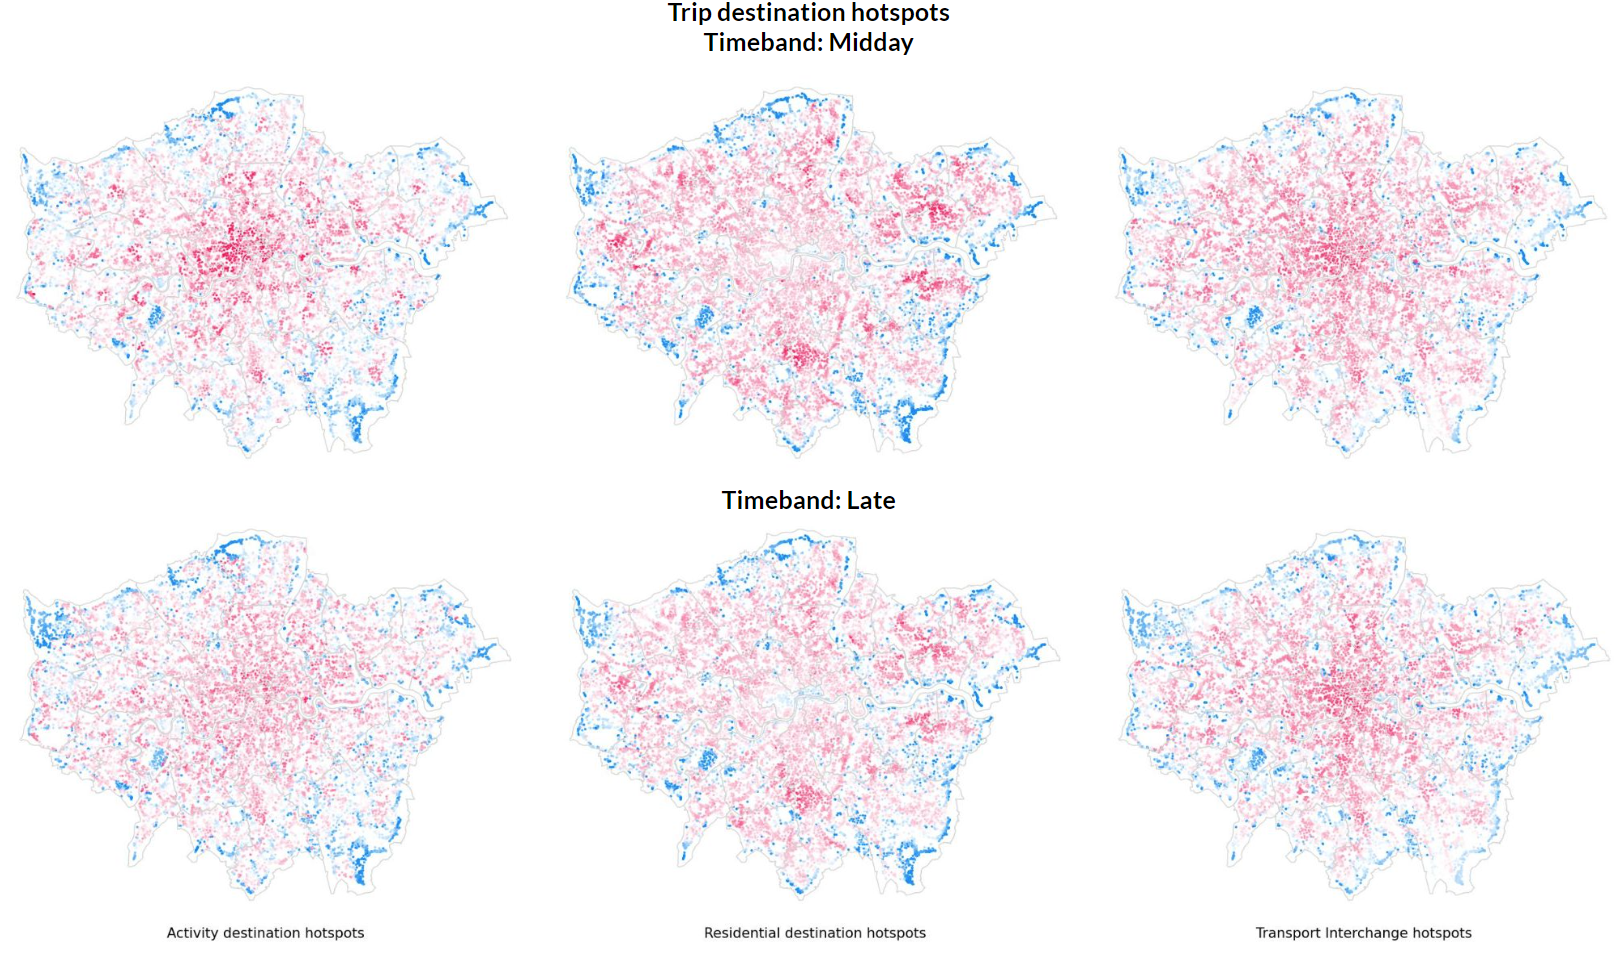
\includegraphics[width=0.75\textwidth]{destinationhotspot.png}
    \captionsetup{justification=centering}
    \caption{Hot spots for destination groups\\ Midday vs Late}
    \label{fig:destinationhotspot}
\end{figure}




\section{Limitations and future work}